\section{Limits on New Physics}
\label{sec:limit}

As discussed in Sec.~\ref{sec:results}, we do not observe any excess in the signal regions.
We use these results to place Bayesian 95\% confidence level upper limits~\cite{ref:cl95cms} on 
the non-SM contributions to the yields in the signal regions, using a log-normal model
of nuissance parameter integration. The results are summarized in Table~\ref{resultsyieldtable}.  

\begin{figure}[hbt]
\begin{center}
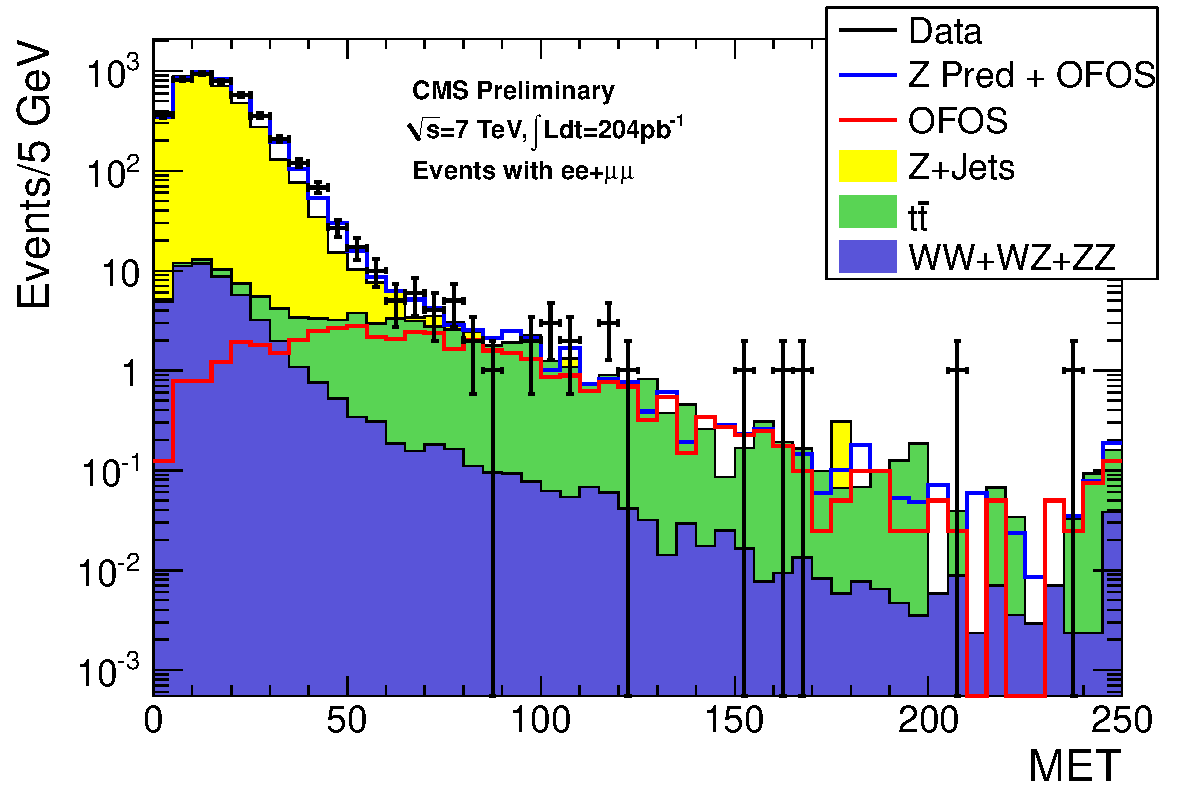
\includegraphics[width=0.78\linewidth]{plots/lep_metPredicted.pdf}
\caption{\label{fig:results}\protect 
  The observed MET distribution for data in the (black points),
  predicted $t\bar{t}$ MET distribution (red line), the sum of predicted %
  $t\bar{t}$ MET distribution and
  $Z$  MET  distribution  predicted  from photon  MET  templates
  (solid blue line),  and MC (solid histograms). 
  }
\end{center}
\end{figure}

\begin{table}[htb]
\begin{center}
\caption{\label{resultsyieldtable} 
Summary of the yields in the regions MET $>$ 30, 60, 100 and 200 GeV. The total predicted yield is the sum of the
predicted background from \Z plus jets from the MET templates method (\Z prediction) plus the \ttbar\ contribution
predicted from OF subtraction (\ttbar\ prediction). Here the first uncertainty is statistical, the second uncertainty is systematic.
The 95\% CL Bayesian UL is indicated, as well as the expected NLO yields for the
LM4 and LM8 scenarios, including the uncertainties from lepton identification and isolation efficiency,
trigger efficiency, hadronic energy scale, and integrated luminosity.
}
\begin{tabular}{lcccc}
\hline
                  &   N(MET $>30$)  GeV          &   N(MET $>60$)  GeV          &   N(MET $>100$) GeV          &   N(MET $>200$) GeV \\
\hline
$Z$ prediction    & 406.2 $\pm$ 7.1 $\pm$ 101.6  &    13.1 $\pm$ 1.2 $\pm$ 3.3  &     1.4 $\pm$ 0.6 $\pm$ 0.4  &     0.05 $\pm$ 0.02 $\pm$ 0.01  \\
\ttbar prediction &  54.8 $\pm$ 3.0 $\pm$ 2.0    &    34.7 $\pm$ 2.4 $\pm$ 1.3  &    11.8 $\pm$ 1.4 $\pm$ 0.4  &      1.1 $\pm$  0.5 $\pm$ 0.04  \\
total prediction  & 461.0 $\pm$ 7.7 $\pm$ 101.6  &    47.9 $\pm$ 2.7 $\pm$ 3.5  &    13.2 $\pm$ 1.5 $\pm$ 0.6  &      1.2 $\pm$  0.5 $\pm$ 0.04  \\
      observed    &                         488  &                          39  &                          14  &                    2            \\
UL                &                         179  &                        11.5  &                        10.0  &                   5.3           \\
LM4               &   5.6 $\pm$ 0.3              &     5.0 $\pm$ 0.3            &     4.4 $\pm$ 0.3            &      2.7 $\pm$ 0.3              \\
LM8               &   2.6 $\pm$ 0.2              &     2.4 $\pm$ 0.2            &     1.9 $\pm$ 0.1            &      1.1 $\pm$ 0.1              \\

\hline
\end{tabular}
\end{center}
\end{table}

